\section{Closing}



%%%%%%%%%%%%%%%%%%%%%%%%%%%%%%%%%%%%%%%%%%%%%%
% \begin{frame}[label=ladila]{Philosophy}

% KT sits naturally in the context of \textbf{panpsychism} (`mind is everywhere', see Strawson, \cite{Goff:2019aa}), a somewhat controversial version of the philosophy of consciousness.  \vfill

% \textbf{Idealism} is perhaps a more rigorous philosophical background (consciousness as the fundamental entity, `mind is everything'). \vfill

%  Although not necessary for the exploration of the scientific implications of the theory, the adoption of idealism can itself be motivated by simplicity and consistency criteria \citep{Symes2022-ri}.
 
% \end{frame}



%%%%%%%%%%%%%%%%%%%%%%%%%%%%%%%%%%%%%%%%%%%%%%%%%%
\begin{frame}[label=ladila]{Neurobiology}
 \begin{center}
  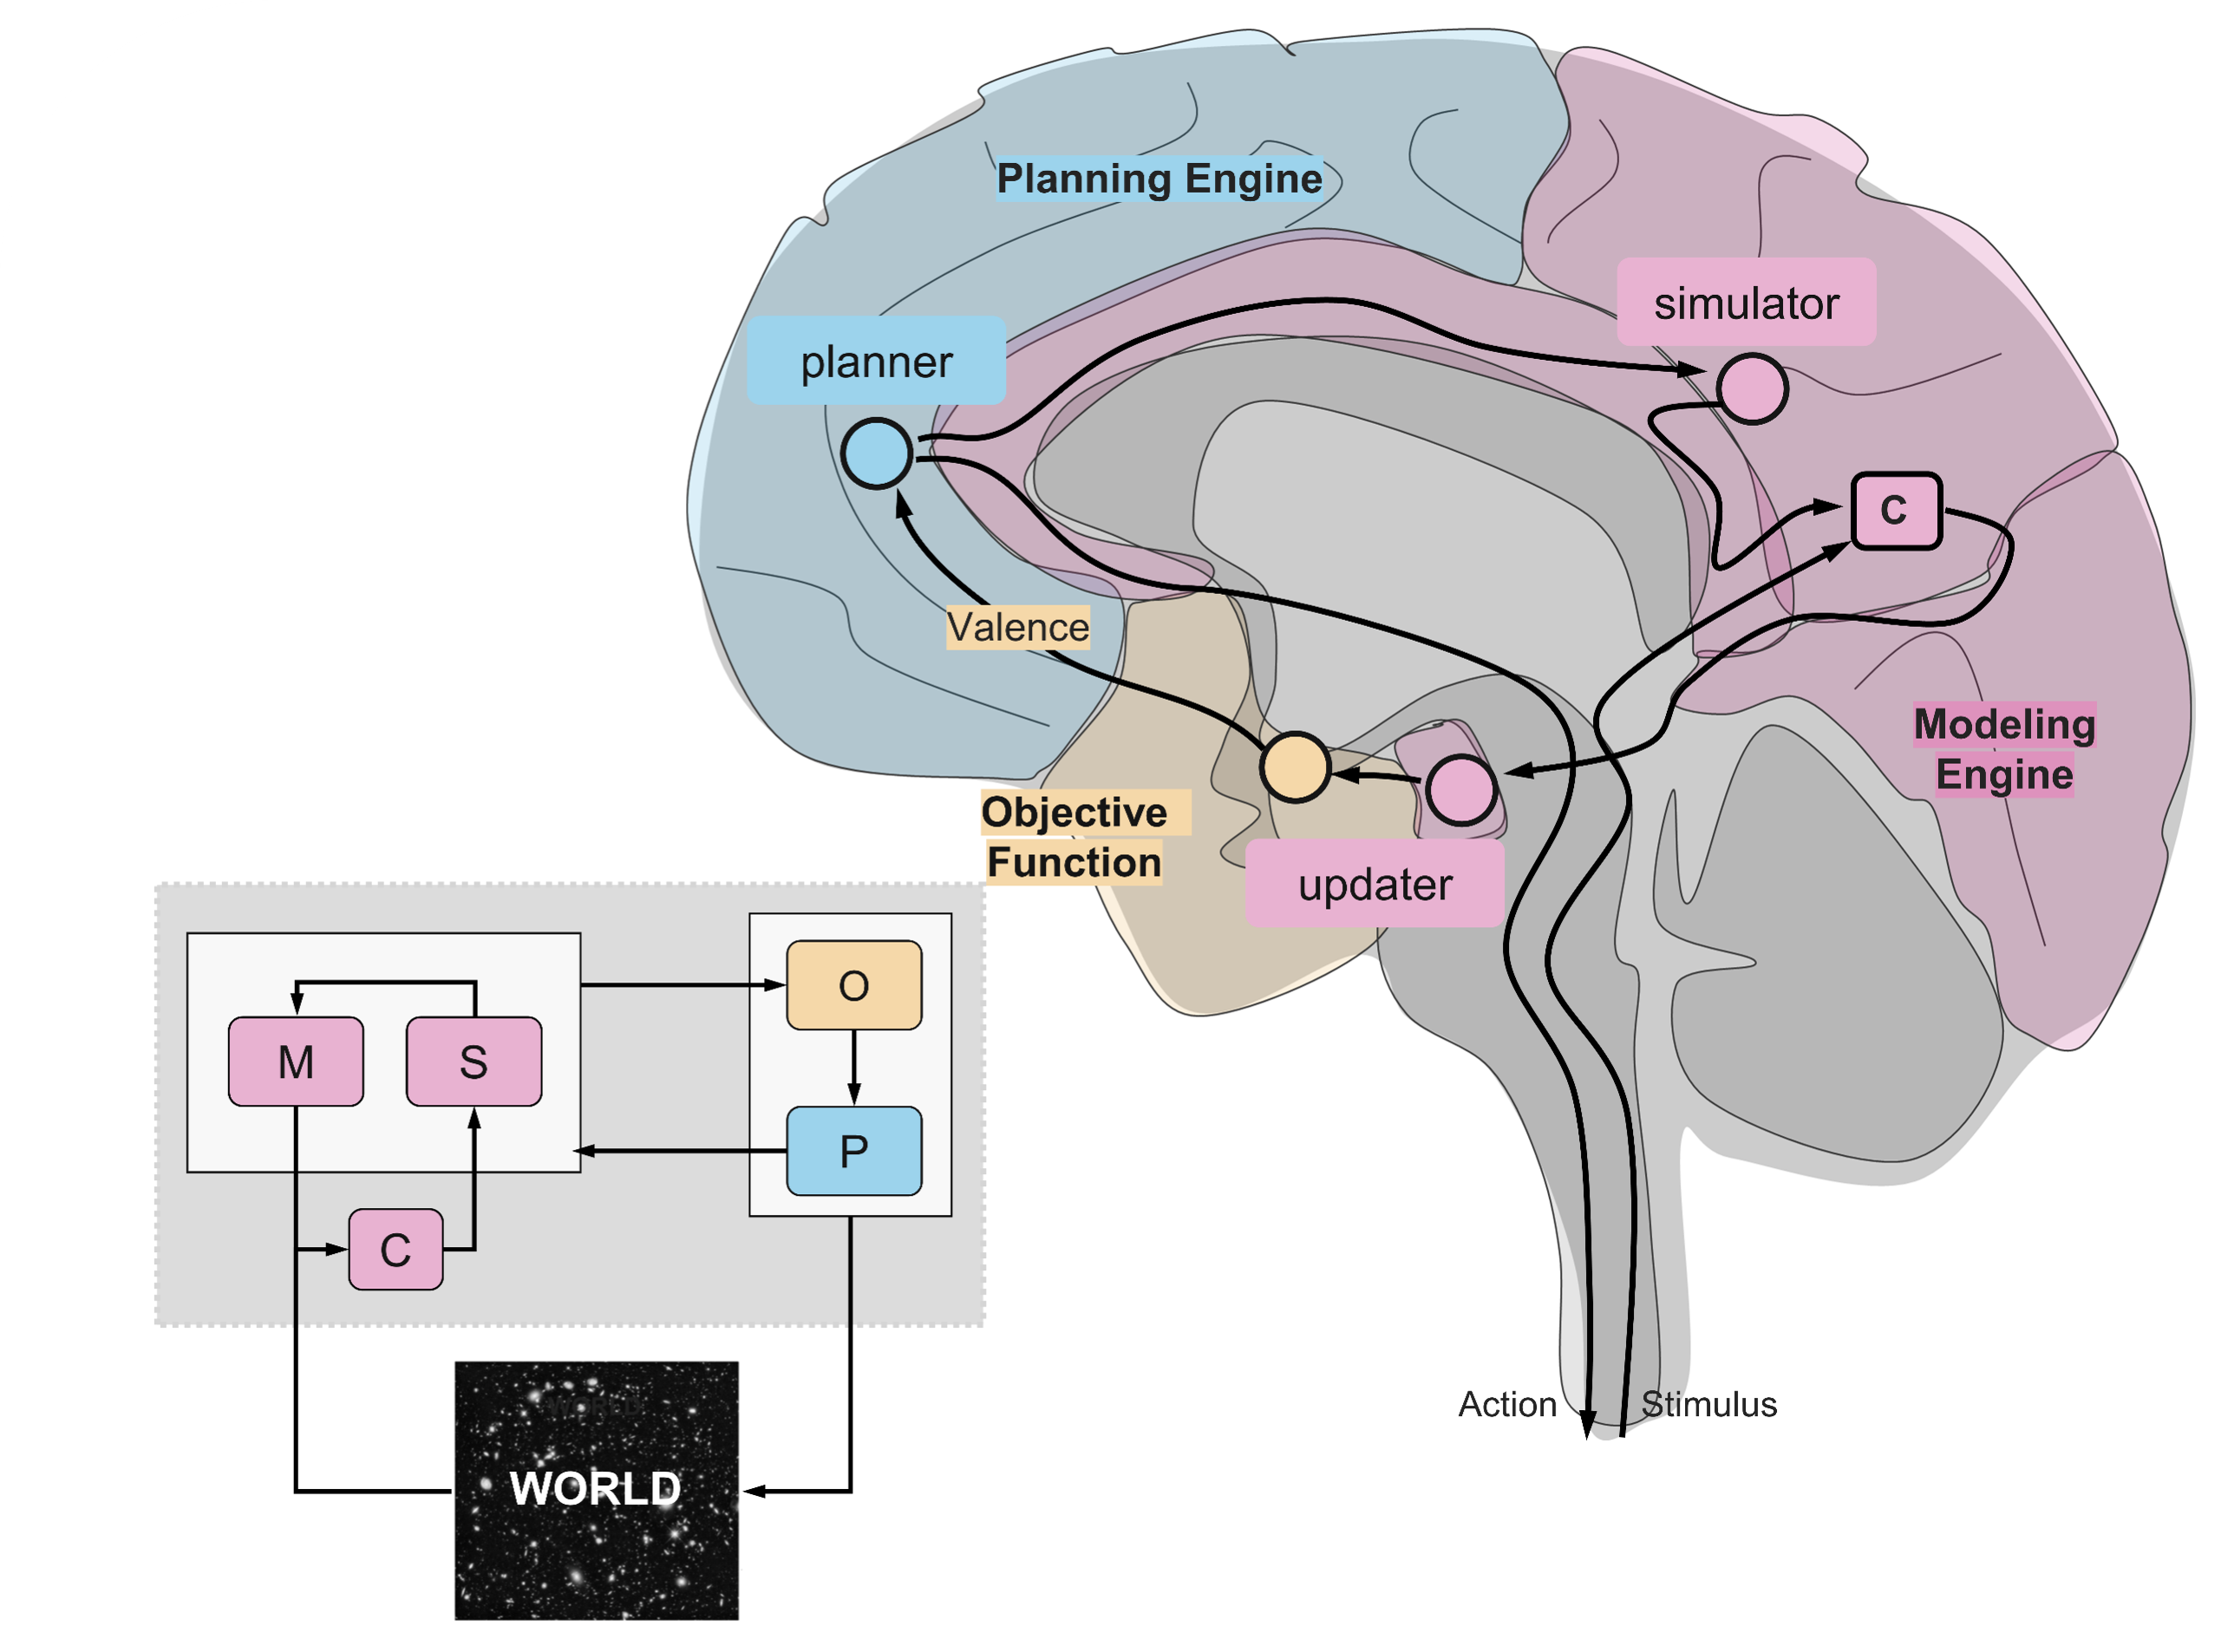
\includegraphics[height=6cm]{img/agent_neuro.png}
  \end{center}

\end{frame}

%%%%%%%%%%%%%%%%%%%%%%%%%%%%%%%%%%%%%%%%%%%%%%%%%%
\begin{frame}[label=ladila]{Neurobiology}
%Theories of cortical processing emphasize the separation of forward and backward information flow in the cortex also mirrored at the level of single cortical pyramidal cells \citep{CarhartHarris2019,Aru2020}. 

The \textbf{Comparator}, crucial for \SEP, is implemented hierarchically in L5 P cells\citep{CarhartHarris2019,Aru2020} (posterior hot zone). \vspace{0.5cm}

 
  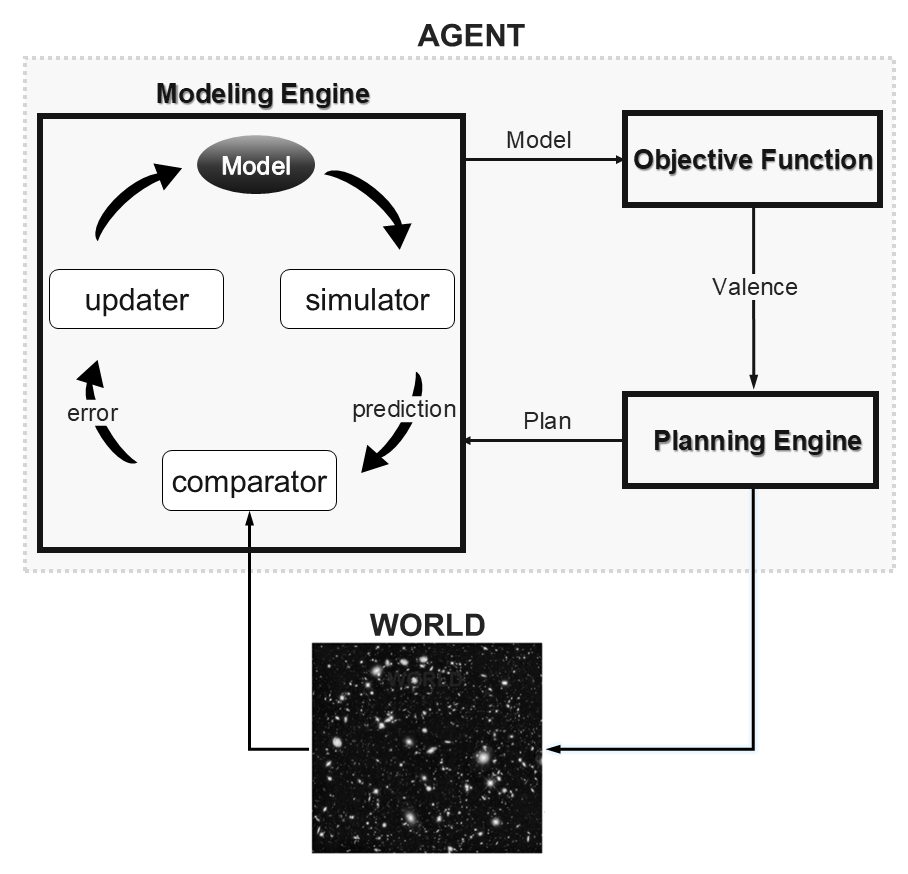
\includegraphics[height=4.cm]{img/Figure1_StructuredDynamics.png}
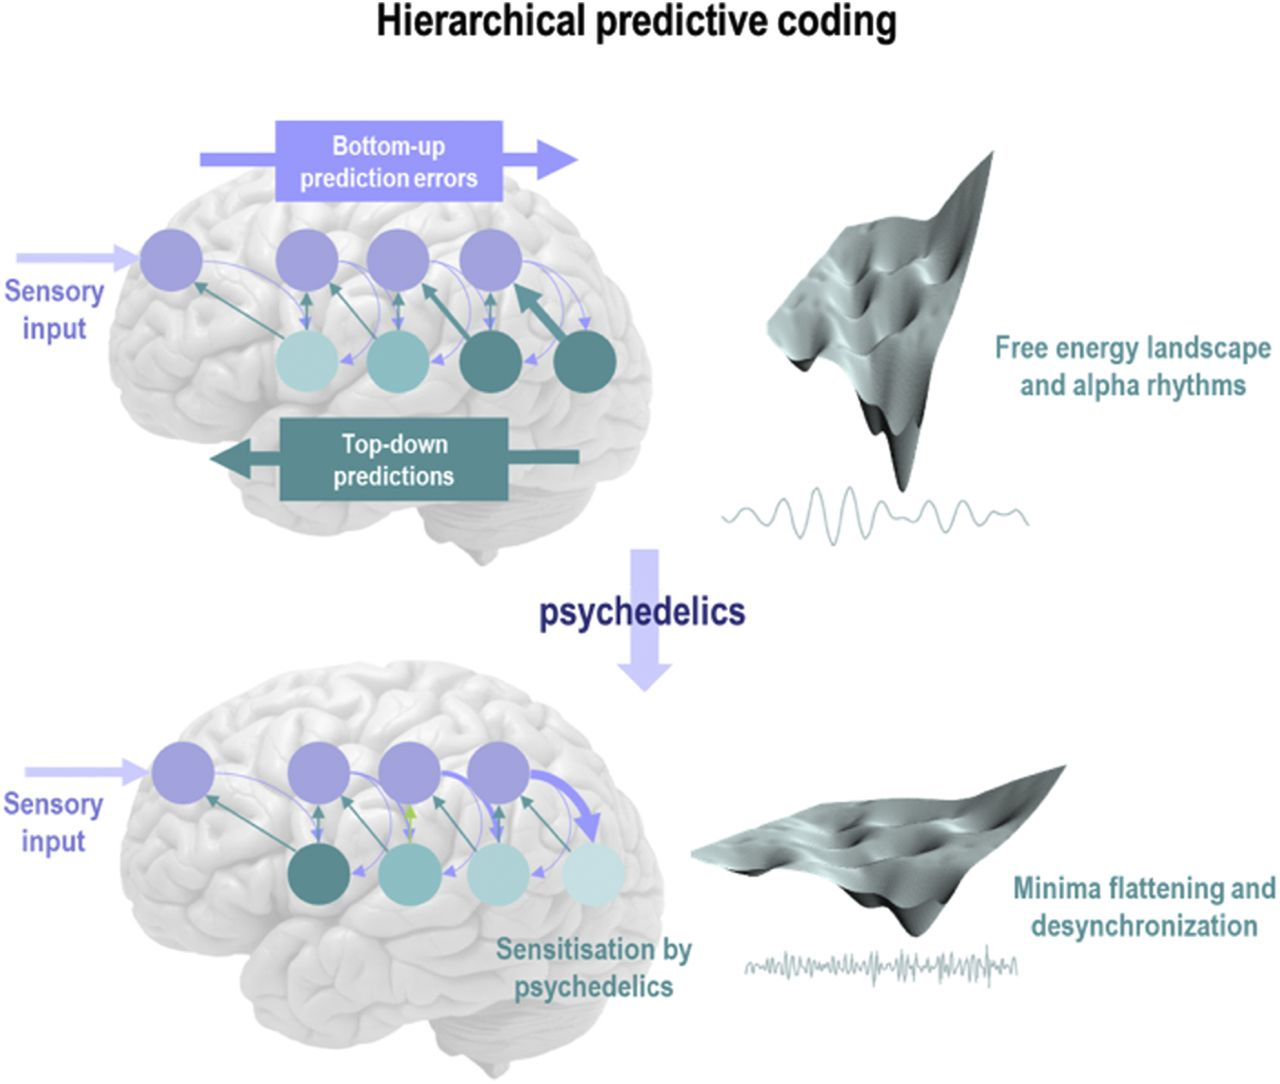
\includegraphics[height=4.cm]{img/F1.large.jpg}
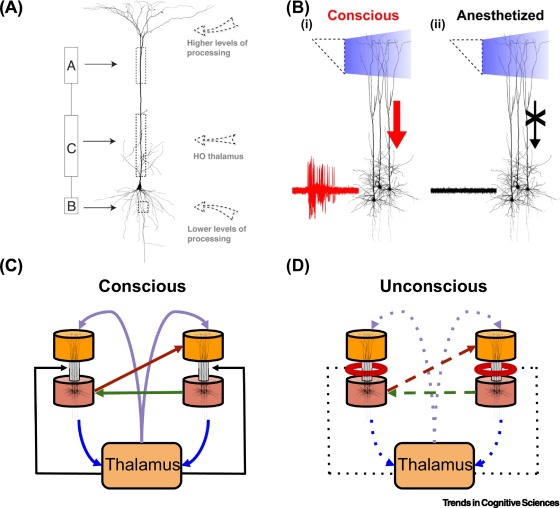
\includegraphics[height=4.cm]{img/gr2.jpeg}
\end{frame}

%%%%%%%%%%%%%%%%%%%%%%%%%%%%%%%%%%%%%%%%%%%%%%


\begin{frame}[label=ladila]{Ethics}
 %To be connected with (neuro)biology.
 KT does not grant any special status to humans:  all \textbf{agents} enjoy structured experience with  \textbf{pleasure/pain (valence)}. \vfill
 \begin{center}
  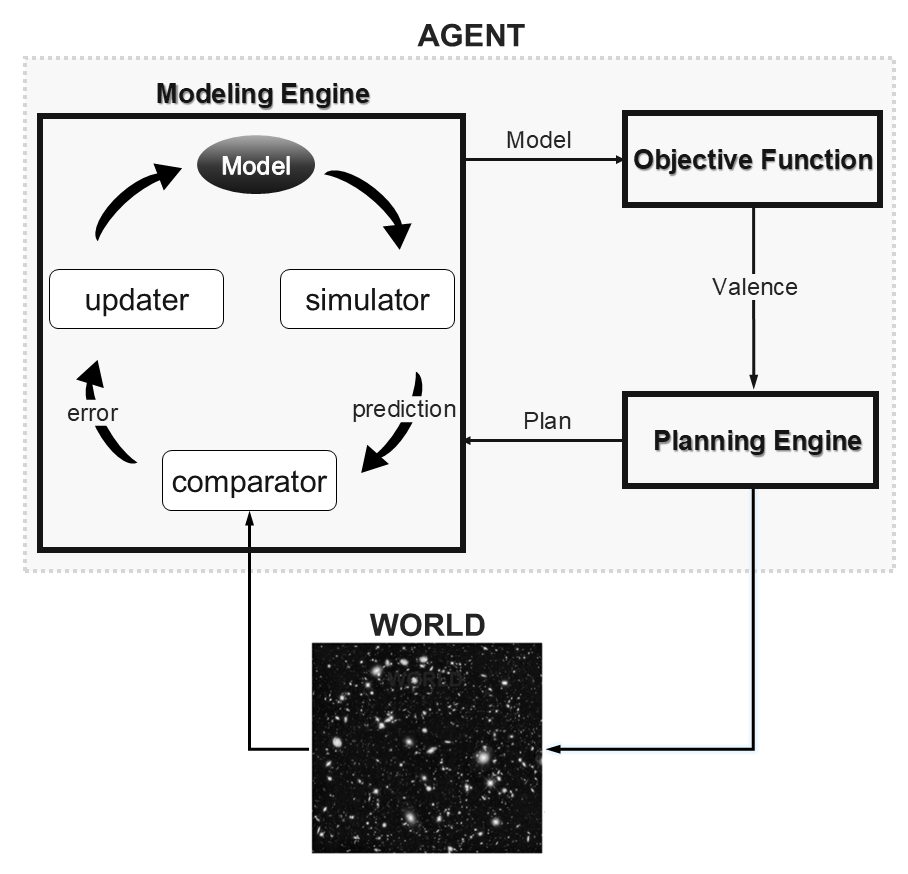
\includegraphics[height=6cm]{img/Figure1_StructuredDynamics.png}
  \end{center}

\end{frame}



\begin{frame}[label=ladila]{Ethics}


The framework has other implications. E.g.,  \textit{morality}:  natural notions of {\em good} or {\em evil} in computational terms. \vfill

E.g., we may say that Agent's $A$ is \textbf{evil} to Agent $B$ if the objective function   $O_A$ increases when O$_B$ decreases, that is $O_A(O_B)$ is decreasing or  $O_A'(O_B) <0$ (and viceversa for \textbf{kind}).
 \vfill
 
% Conversely, we say that Agent $A$ is {\em good or morally right} to Agent $B$ if $O_A'(O_B) >0$. \vfill 

%Synergistic behavior emerges when agents are \textit{kind} to each other, while mutually-destructive behavior takes place in the complementary case.  
 
\end{frame}


\begin{frame}[label=ladila]{Emotion \cite{ruffini_algorithmic_2024}}
 
   To include the experience dimension of \textbf{valence} in the agent, we define: 
\begin{definition}[Emotional state or Mood of an Agent] 
The {\bf emotional state} of the Agent is the tuple E = (Model, Valence). 
\end{definition}
In first-person language, {\em emotion is structured experience with valence}, and can be described along dimensions characterizing model structure (simplicity, breadth, accuracy, etc.) plus valence.  
  \begin{definition}[Depressed Agent] 
{\bf Depression} is a pathological state in which the output value of the Objective Function (valence) of an agent is persistently low.
\end{definition}
    
 
\end{frame}


%%%%%%%%%%%%%%%%%%%%%%%%%%%%%%%%%
\begin{frame}[label=ladila]{Future}
% Firmly reconcile KT with AIF/FEP, IIT, GWT, DIT. 
 % \vfill
 

Demonstrate how to computationally \textit{evolve agents}. KT conjecture: \textit{\textit{Under some conditions, persistent patterns} are unavoidable  in a computational soup if we wait long enough.} Are there patterns other than agents  (life/intelligence)? \vfill

How can we detect an agent through its behavior or structure? \vfill


How can we associate the structure of dynamical hierarchical reduced manifolds\cite{ruffini_algorithmic_2024} with first and third-person data?\vfill

Use AI to design better neurophenomenological methods to study \SEP.   \vfill

Map the neurobiology of agenthood\cite{ruffini_algorithmic_2024}?\vfill

Design model-building agents mimicking life or intelligence. 
 
\end{frame}


\begin{frame}{Call for papers: Special Entropy issue}

\begin{figure}
        \centering
        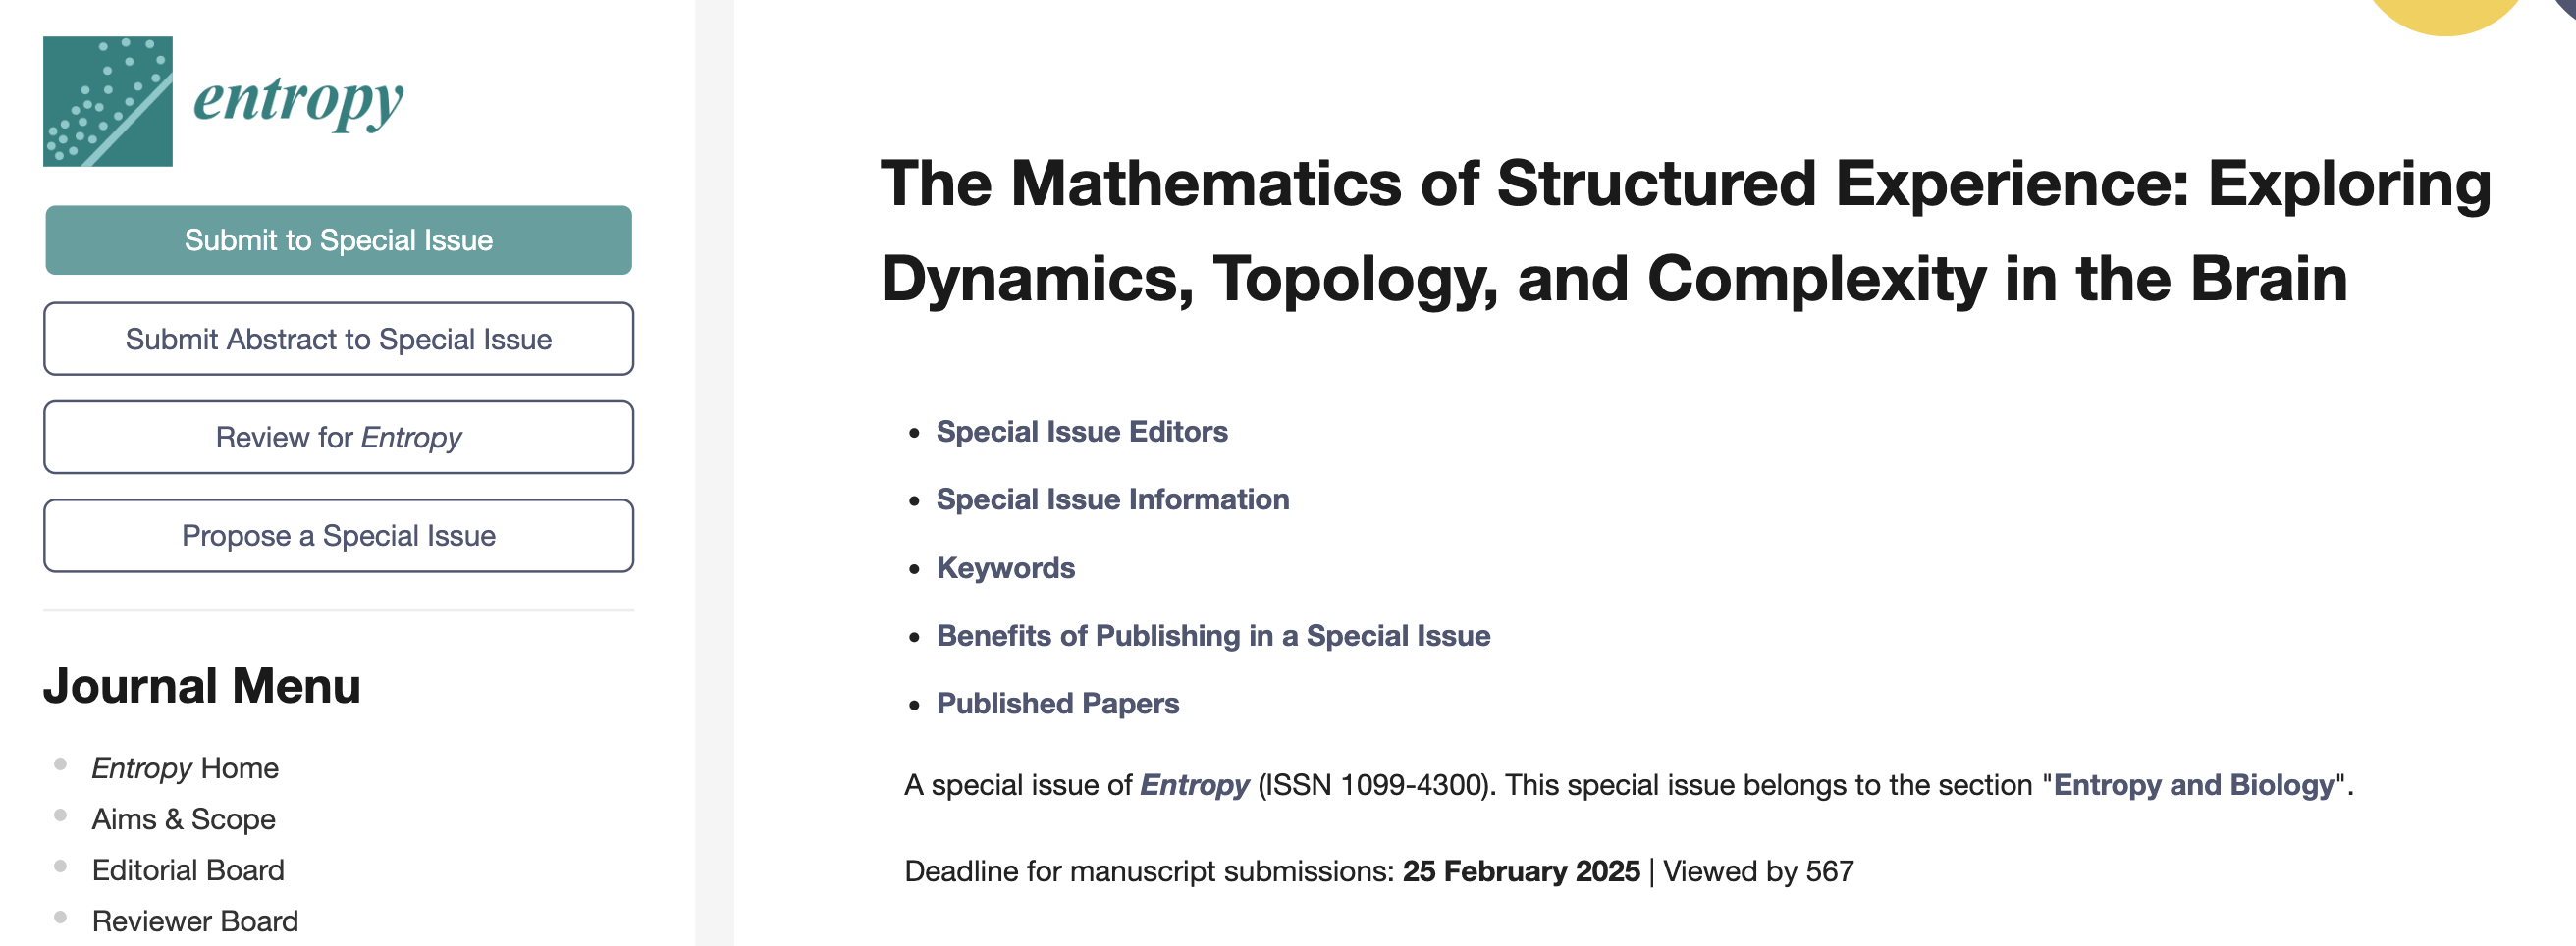
\includegraphics[width=0.81\linewidth]{image8b.png}
        \end{figure}
     
        
   % Titled “The Mathematics of Structured Experience: Exploring Dynamics, Topology, and Complexity in the Brain”, this Special Issue aims to explore several key areas in this program:

%Characteristics of compressive world models;  We aim to delve into the nature of the world models created and run by natural and artificial agents. What do we mean, precisely, by a world model? What is the connection between program structure and the resulting dynamics? What is the role of symmetry and criticality in shaping world models and programs, and how do they enable agents to encapsulate the world's complexity in a comprehensible form?
 

\begin{tcolorbox}[colback=gray!10, colframe=gray!70, title={Topics}]
  Characteristics of compressive world models; Mapping models to dynamical systems;  
Empirical paradigms; 
AI and computational  brain modeling. 
\end{tcolorbox}
\end{frame}


%%%%%%%%%%%%%%%%%%%%%%%%%%%%%%%%%
\begin{frame}[label=ladila]{Thanks}
\vfill
\begin{center}

   {\Large Thanks for your attention and curiosity!}  \vfill
   
  % {\large Thanks to  Ed and Roser for all the brainstorming.}  \vfill
    

    
    Slides available at {\small  %https://github.com/giulioruffini/Ruffini-KT-Tucson-presentation-April-19-2022
    https://github.com/giulioruffini/SLIDES-KT-Bamberg-presentation-Oct-2024} 
    %\\ $\rightarrow$~Preprint is on the way.
    %\vspace{1.5cm} 
    
        %giulio.ruffini@neuroelectrics.com, @ruffini (Twitter)  \vfill
        \begin{figure}
            \centering
            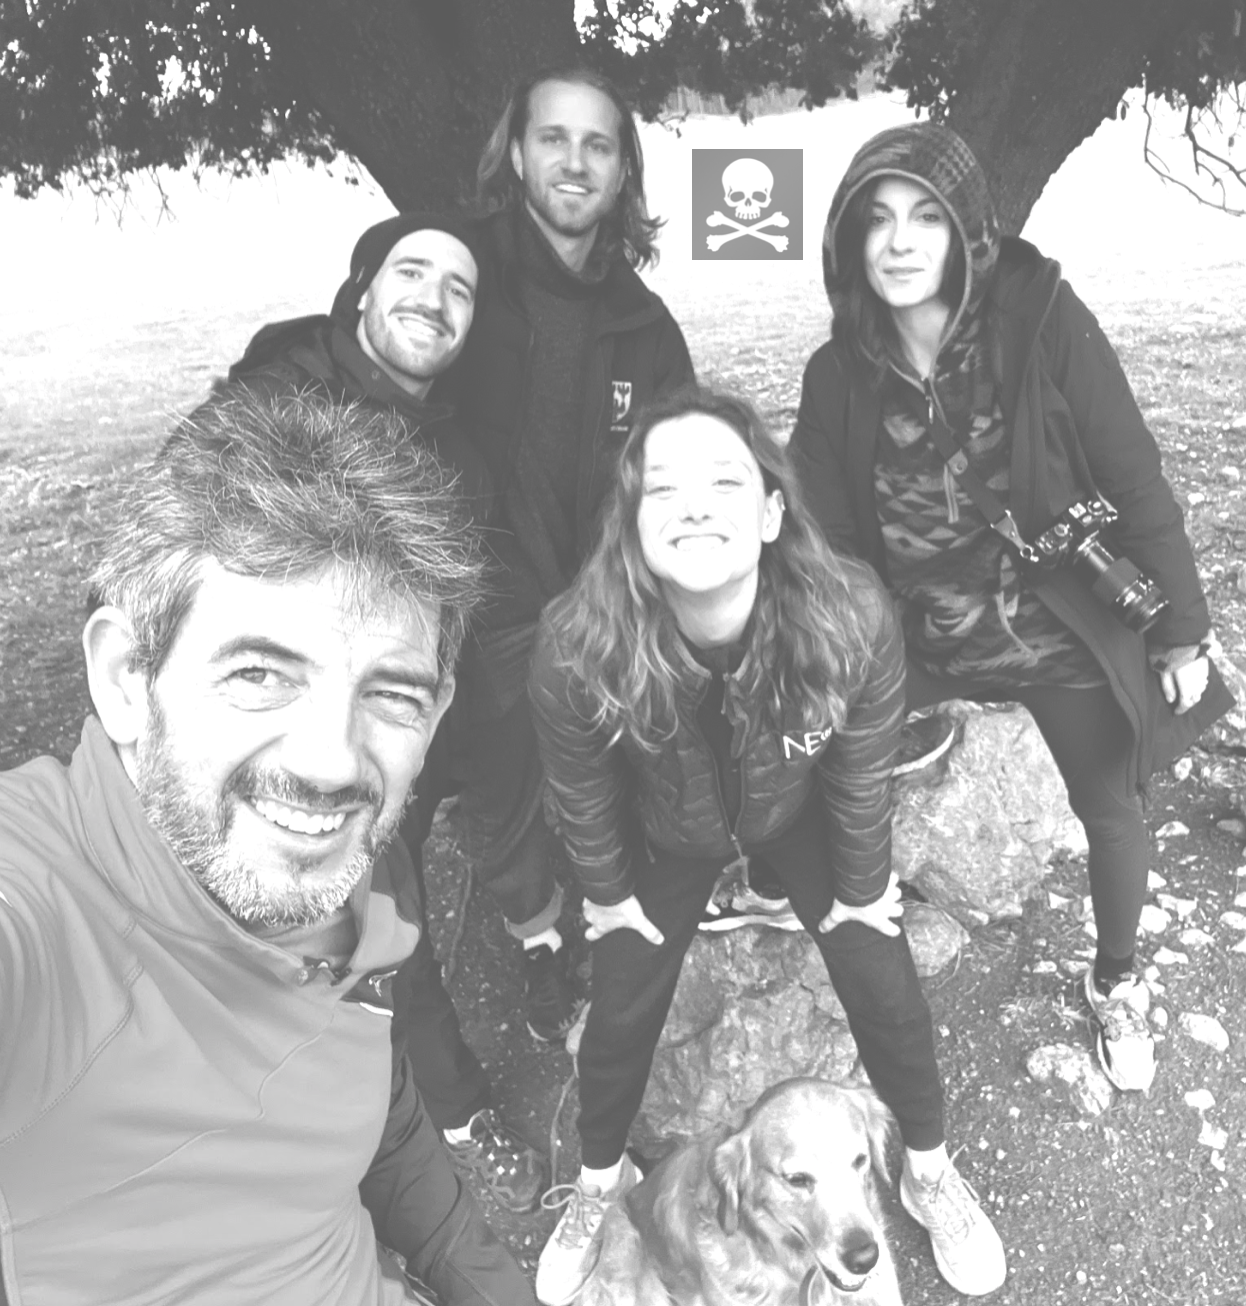
\includegraphics[width=0.33\linewidth]{image2.png}
        \end{figure}
\end{center}
\vfill

\end{frame}